\chapter{Orbits}

A satellite stays in orbit around the planet because the pull of the
planet's gravity causes it to accelerate toward the center of the
planet. 

\begin{figure}[htbp]
    \centering
    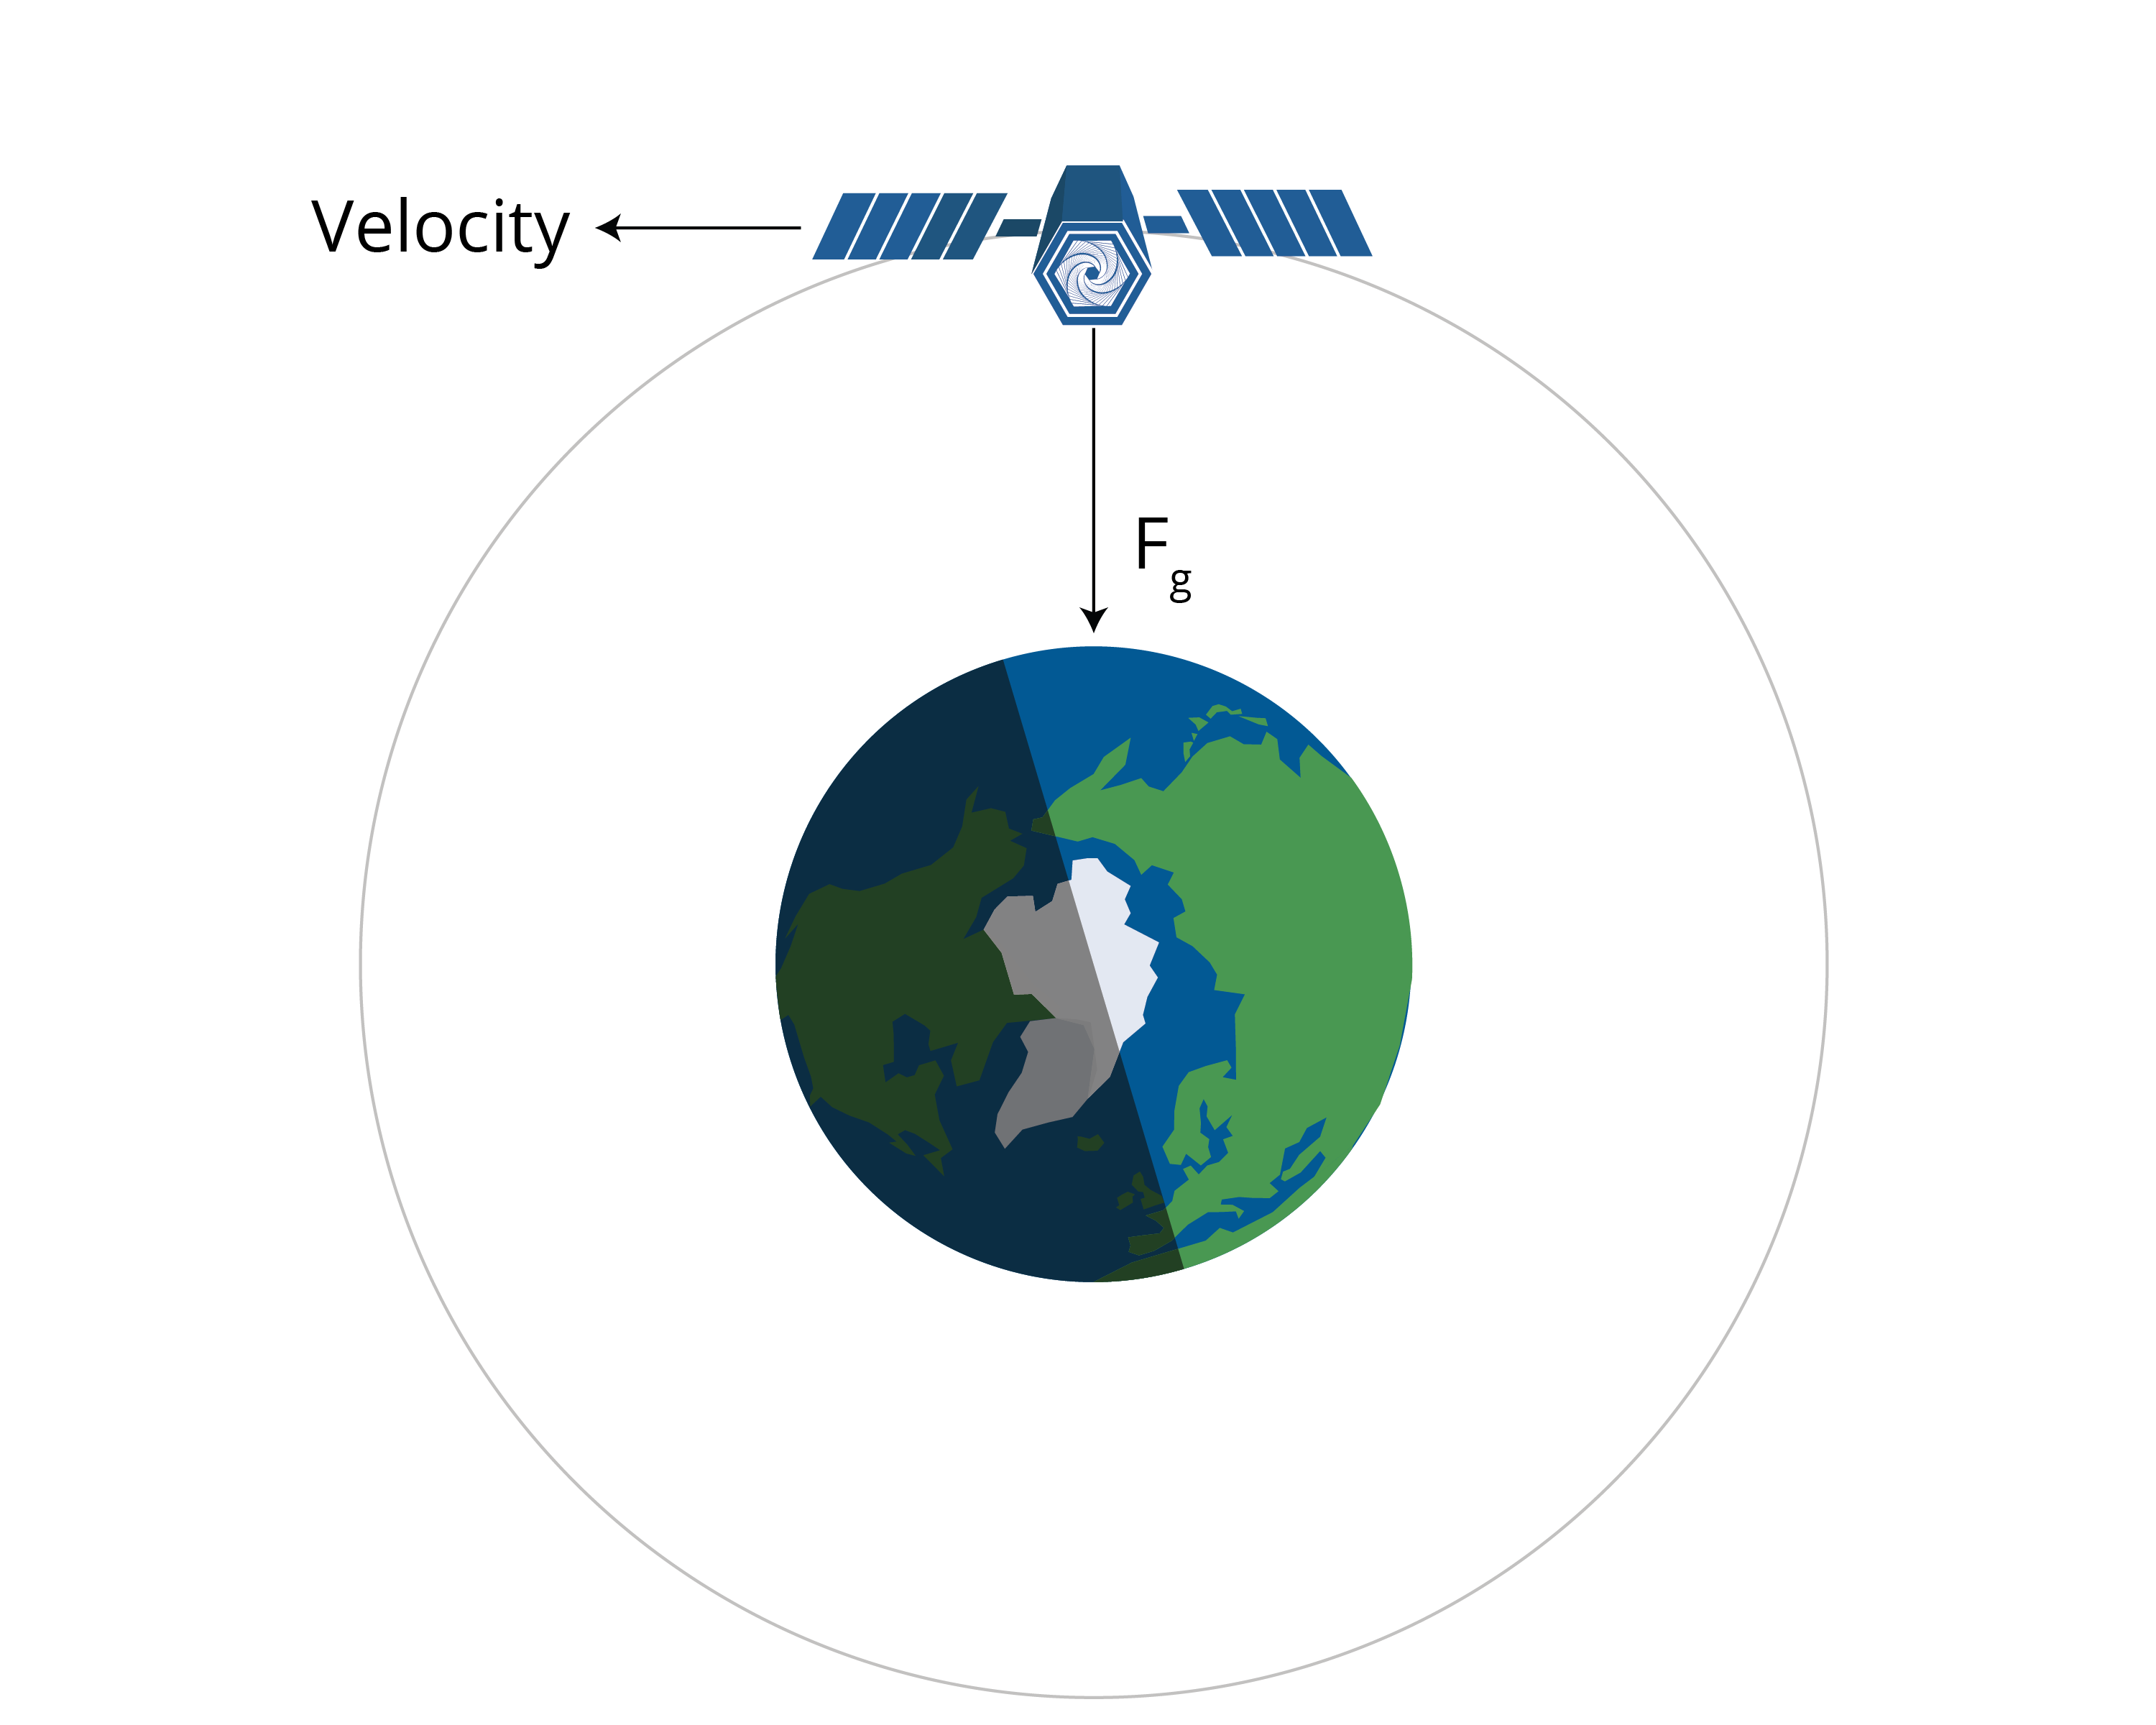
\includegraphics[width=.75\textwidth]{satellite.png}
    \caption{A satellite's centripetal force is gravity.}
    \label{fig:satellite}
\end{figure}


The satellite must be moving at a very particular speed to keep a
constant distance from the planet --- to travel in a circular orbit.
If it is moving too slowly, it will get closer to the planet.  If it
is going too fast, it will get farther from the planet.
\begin{figure}[htbp]
    \centering
    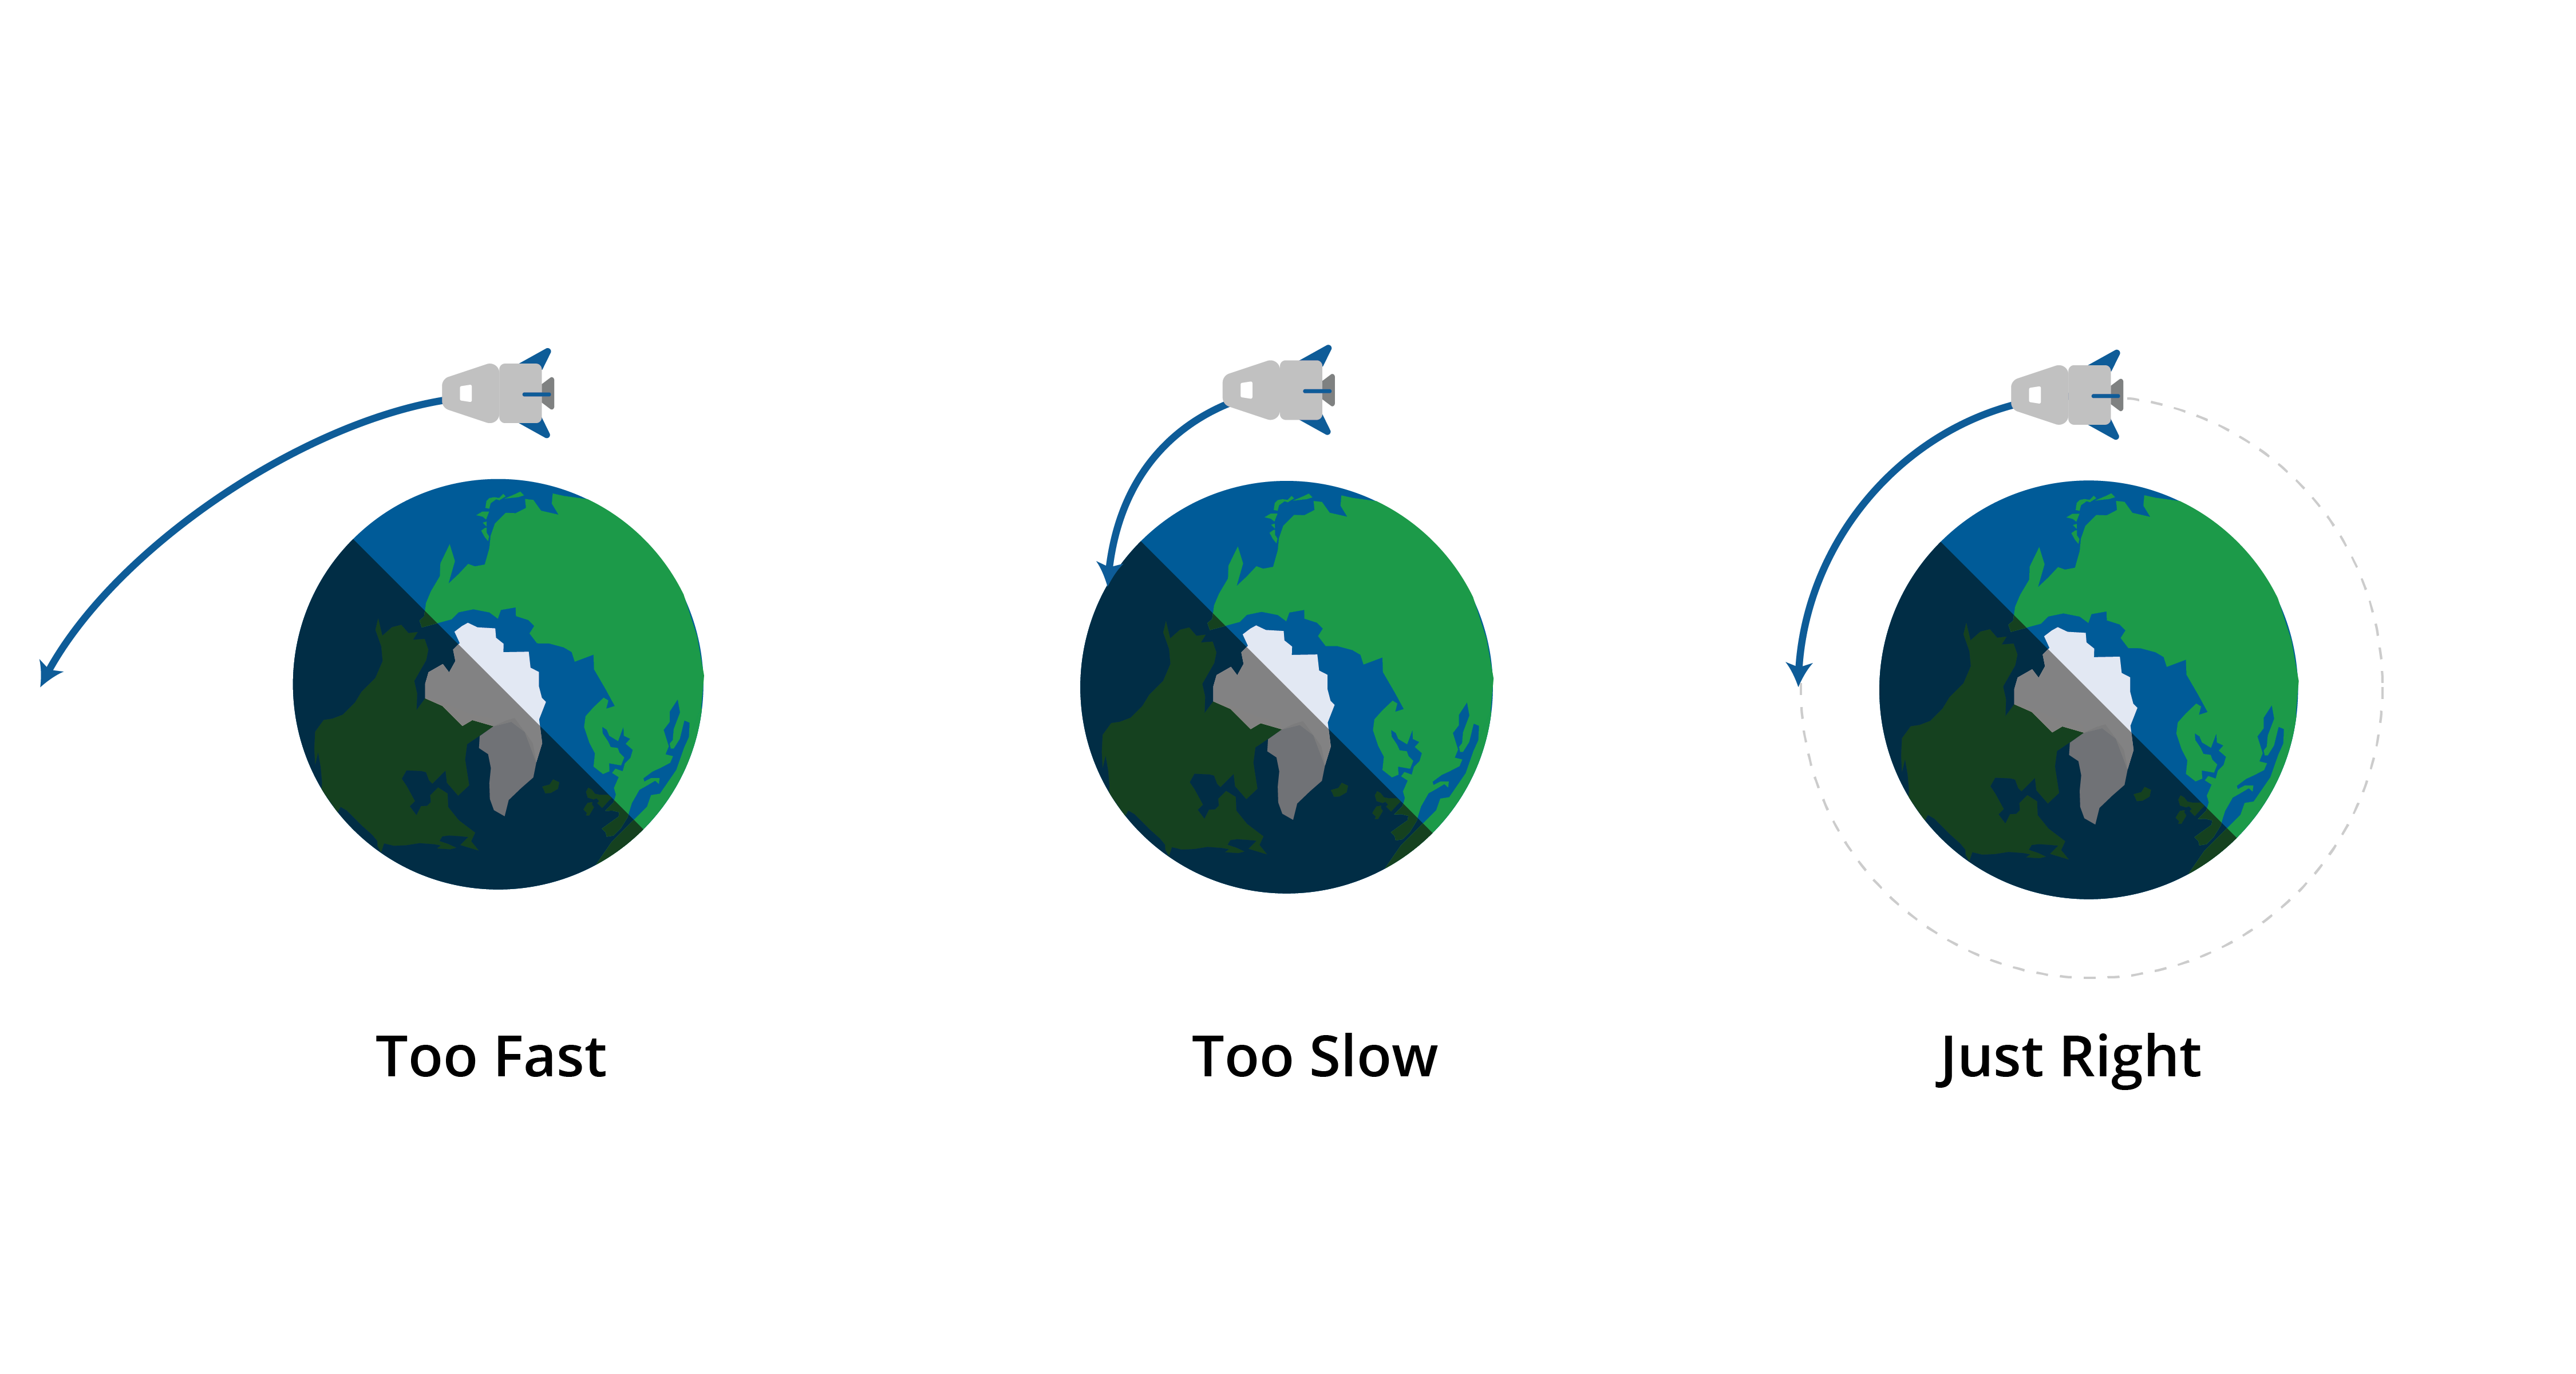
\includegraphics[width=.75\textwidth]{orbitSpeeds.png}
    \caption{A diagram showing the required speeds for entering orbit.}
    \label{fig:orbitSpeeds}
\end{figure}



The radius of the earth is about 6.37 million meters. A satellite that
is in a low orbit is typically about 2 million meters above the
ground. At that distance, the acceleration due to gravity is more like
$6.8 m/s^2$, instead of the $9.8 m/s^2$ that we experience on the
surface of the planet.

How fast does the satellite need to be moving in a circle with a
radius of 8.37 million meters to have an acceleration of $6.8 m/s^2$? Real fast.

Recall that the acceleration vector is

$$a = \frac{v^2}{r}$$

Thus the velocity $v$ needs to be:

$$v = \sqrt{a r} = \sqrt{6.8(8.37 x 10^6)} = 7,544 \text{ m/s}$$

(That's 16,875 miles per hour.)

When a satellite falls out of orbit, it enters the atmosphere at that
7,544 m/s.  The air rushing by generates so much friction that the
satellite gets very, very hot, and usually disintegrates.

\section{Astronauts are \emph{not} weightless}

Some people see astronauts floating inside an orbiting spacecraft and
think there is no gravity: that the astronauts are so far away that
the gravity of the planet doesn't affect them. This is incorrect.  The
gravity might be slightly less (Maybe 6 newtons per kg instead of 9.8
newtons per kg), but the weightless they experience is because they
and the spacecraft is in free fall.  They are just moving so fast (in
a direction perpendicular to gravity) that they don't collide with the
planet.

% 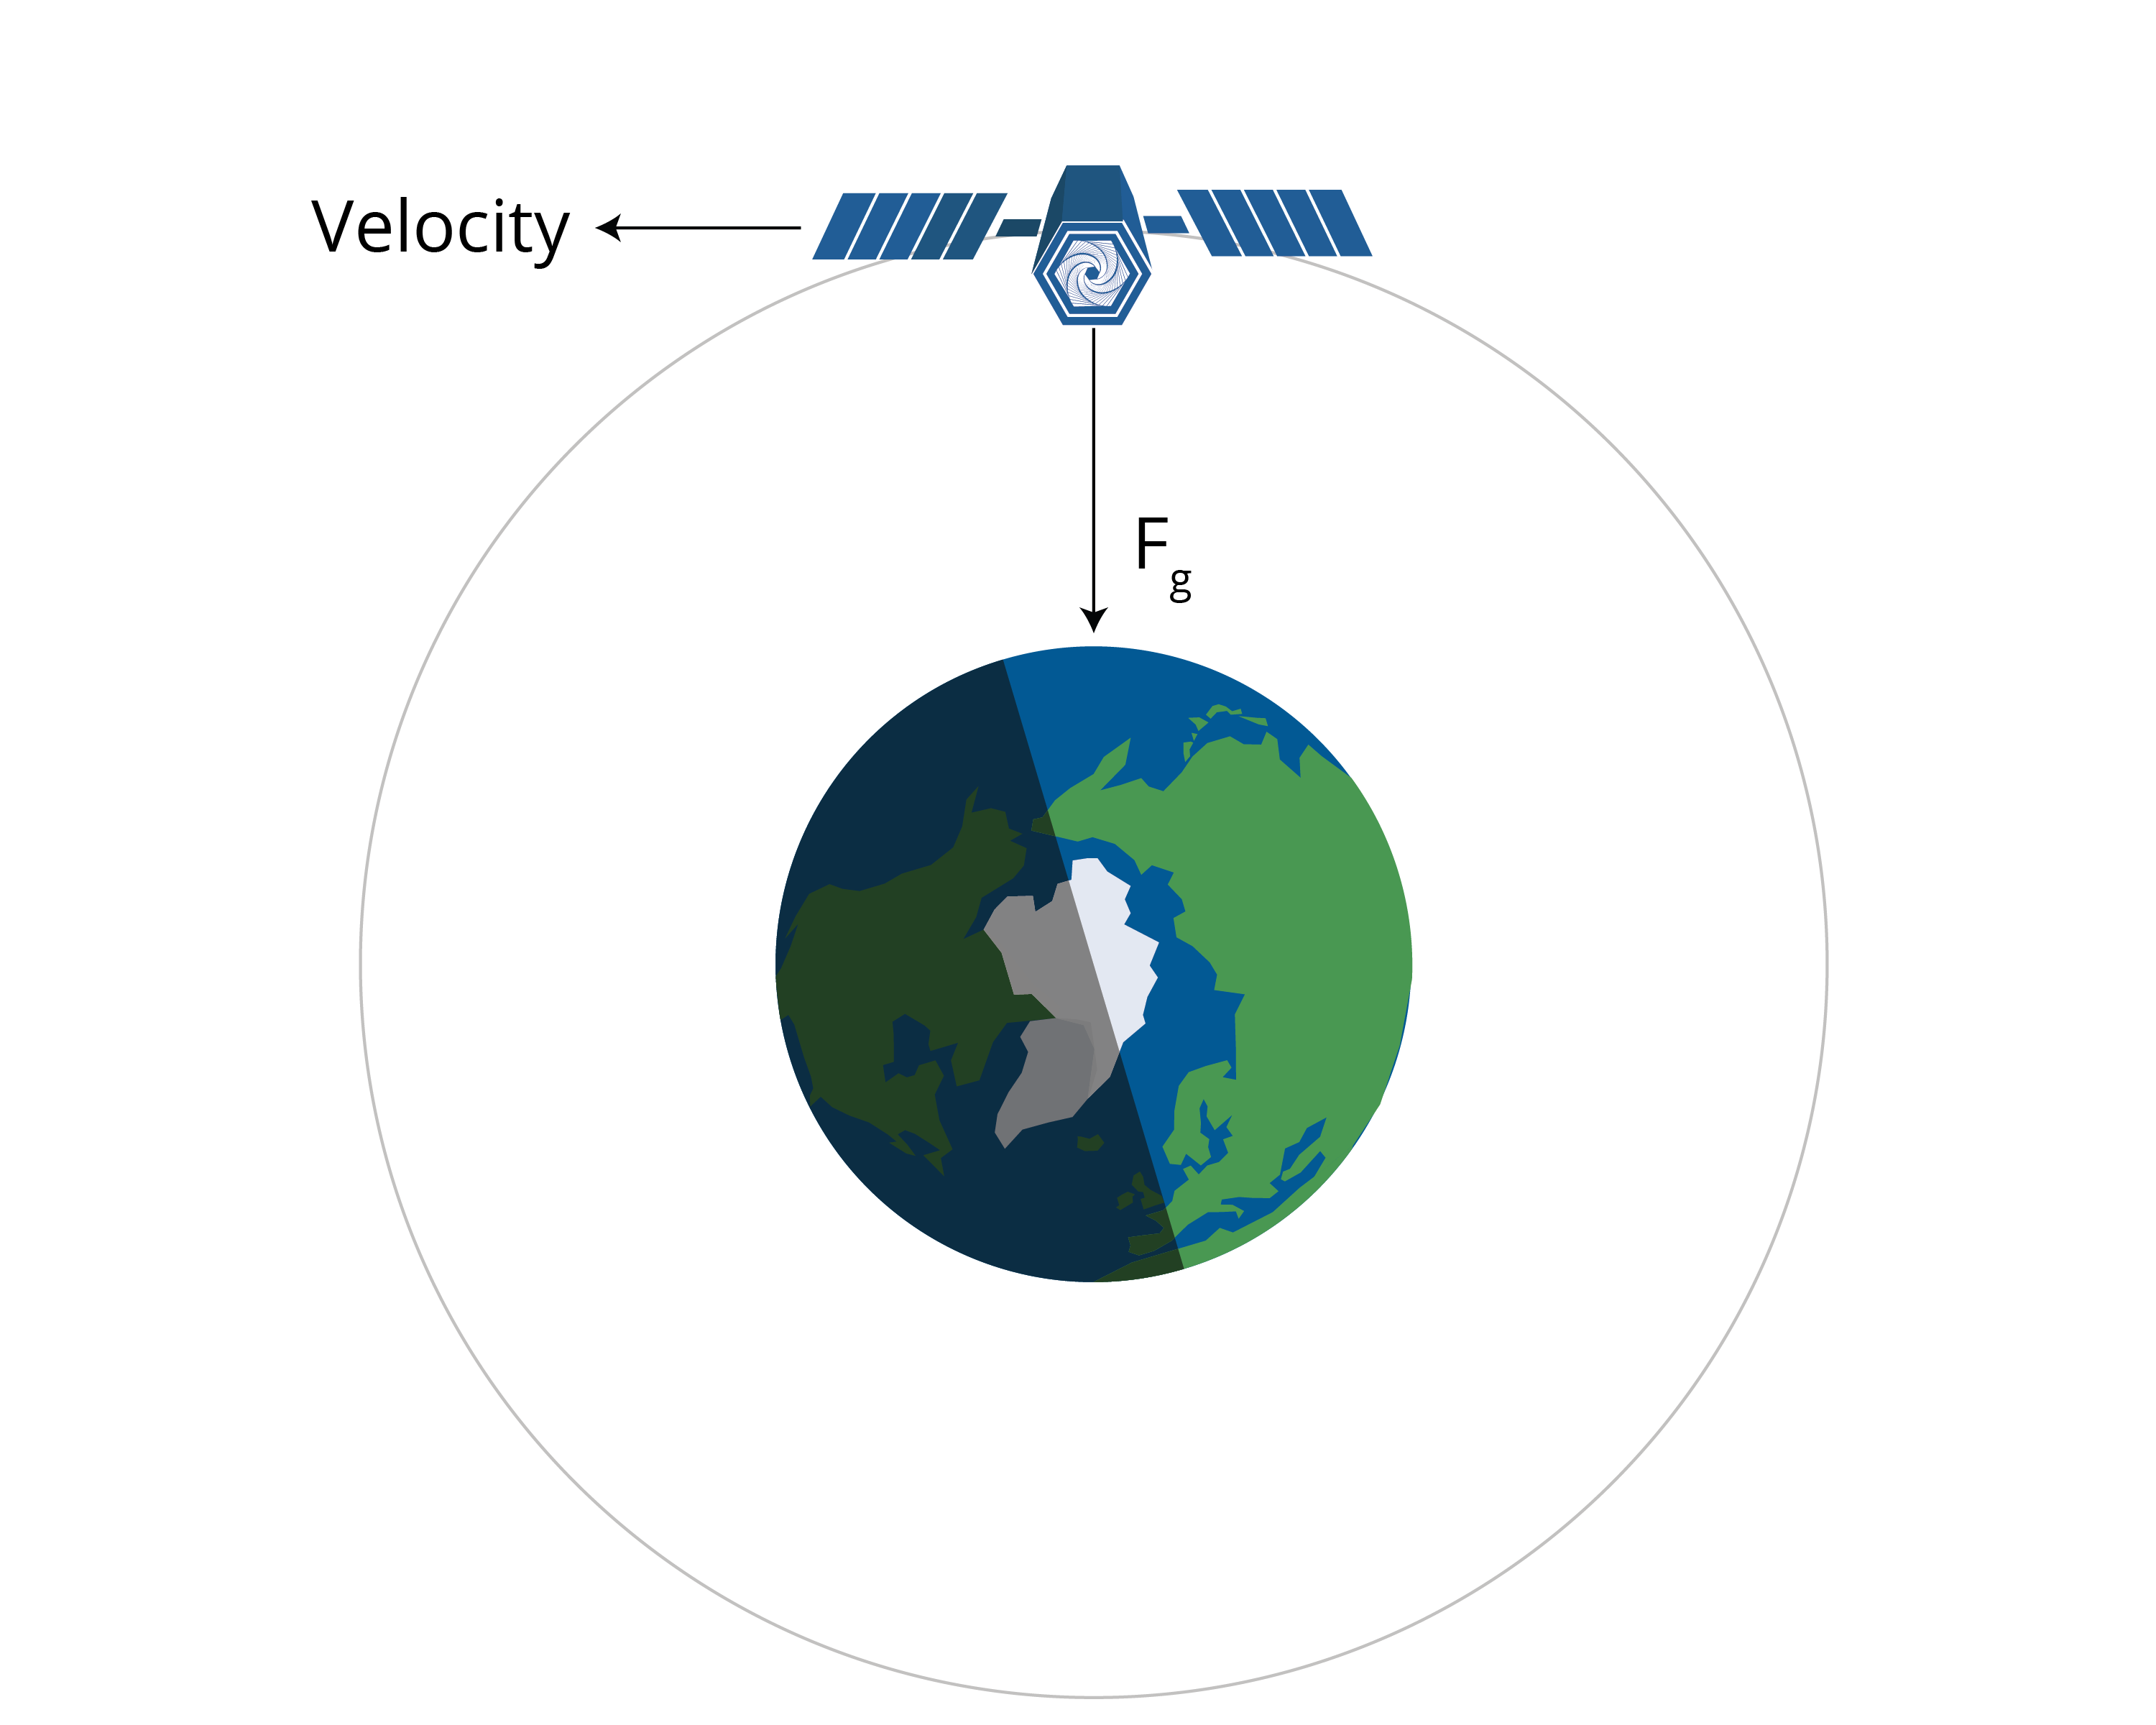
\includegraphics[width=1\textwidth]{satellite.png}


\begin{Exercise}[title={Mars Orbit}, label=mars_orbit]
  
  The radius of Mars is 3.39 million meters. The atmosphere goes up
  another 11 km.  Let's say you want to put a satellite in a circular
  orbit around Mars with a radius of 3.4 million meters.

  The acceleration due to gravity on the surface of Mars is $3.721
  m/s^2$. We can safely assume that it is approximately the same 11 km
  above the surface.

  How fast does the satellite need to be traveling in its orbit?  How
  long will each orbit take?

\end{Exercise}
\begin{Answer}[ref=circular]
  $$v = \sqrt{3.721(3.4 \times 10^6)} = 3,557\text{ m/s}$$

  The circular orbit is $2\pi(3.4 \times 10^6) = 21.4 \times 10^6$ meters in circumference.

  The period of the orbit is $(21.4 \times 10^6)/3,557 \approx 6,000$ seconds.
\end{Answer}

\section{Geosynchronous Orbits}
\index{geosynchronous orbits}
The planet earth rotates once a day.  Satellites in low orbits circle
the earth many times a day. Satellites in very high orbits circle
less than once per day. There is a radius at which a satellite orbits
exactly once per day.  Satellites at this radius are known as
``geosynchronous'' or ``geostationary'', because they are always
directly over a place on the planet.
\begin{figure}[htbp]
    \centering
    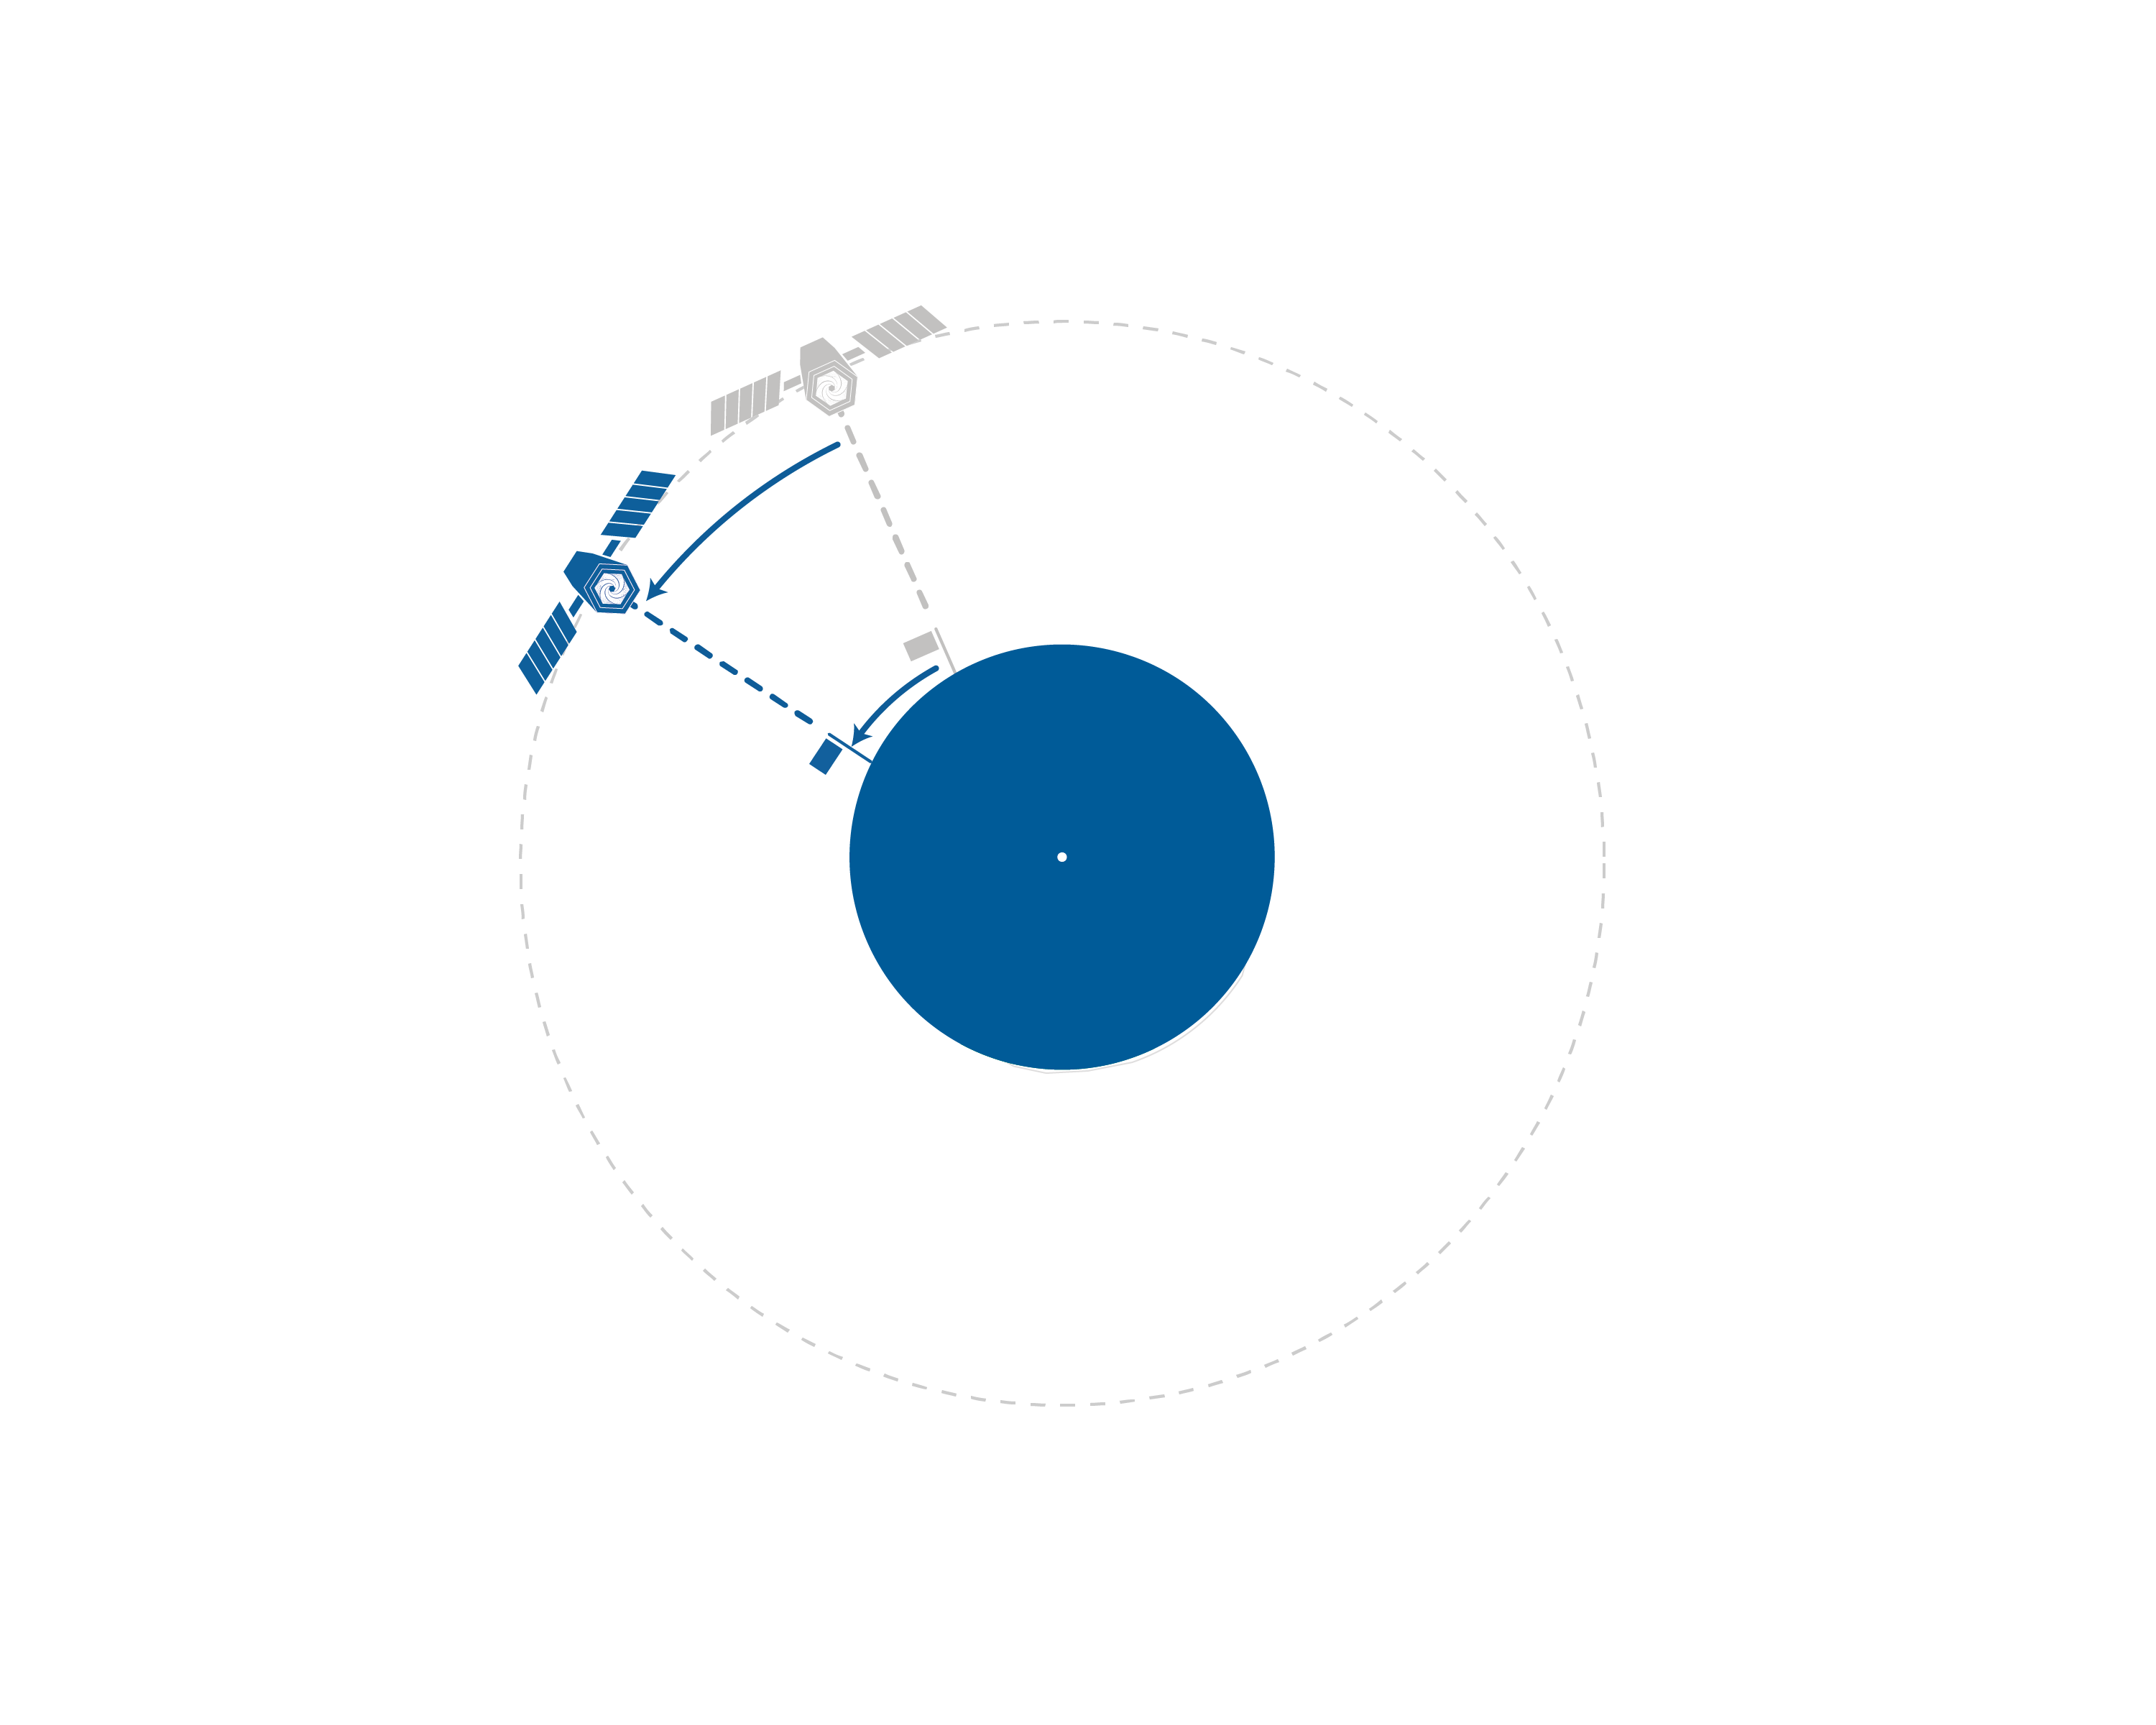
\includegraphics[width=.75\textwidth]{geoSync.png}
    \caption{A satellite in geosynchronous orbit.}
    \label{fig:geoSync}
\end{figure}

The radius of a circular geosynchronous orbit is 42.164 million
meters. (About 36 km above the surface of the earth.)

A geosynchronous satellite travels at a speed of 3,070 m/s.

Geosynchronous satellites are used for the Global Positioning
Satellite system, weather monitoring system, and communications
system.
\section{Escape velocity}
\index{escape velocity}
FIXME: Add text for escape velocity
\begin{figure}[htbp]
    \centering
    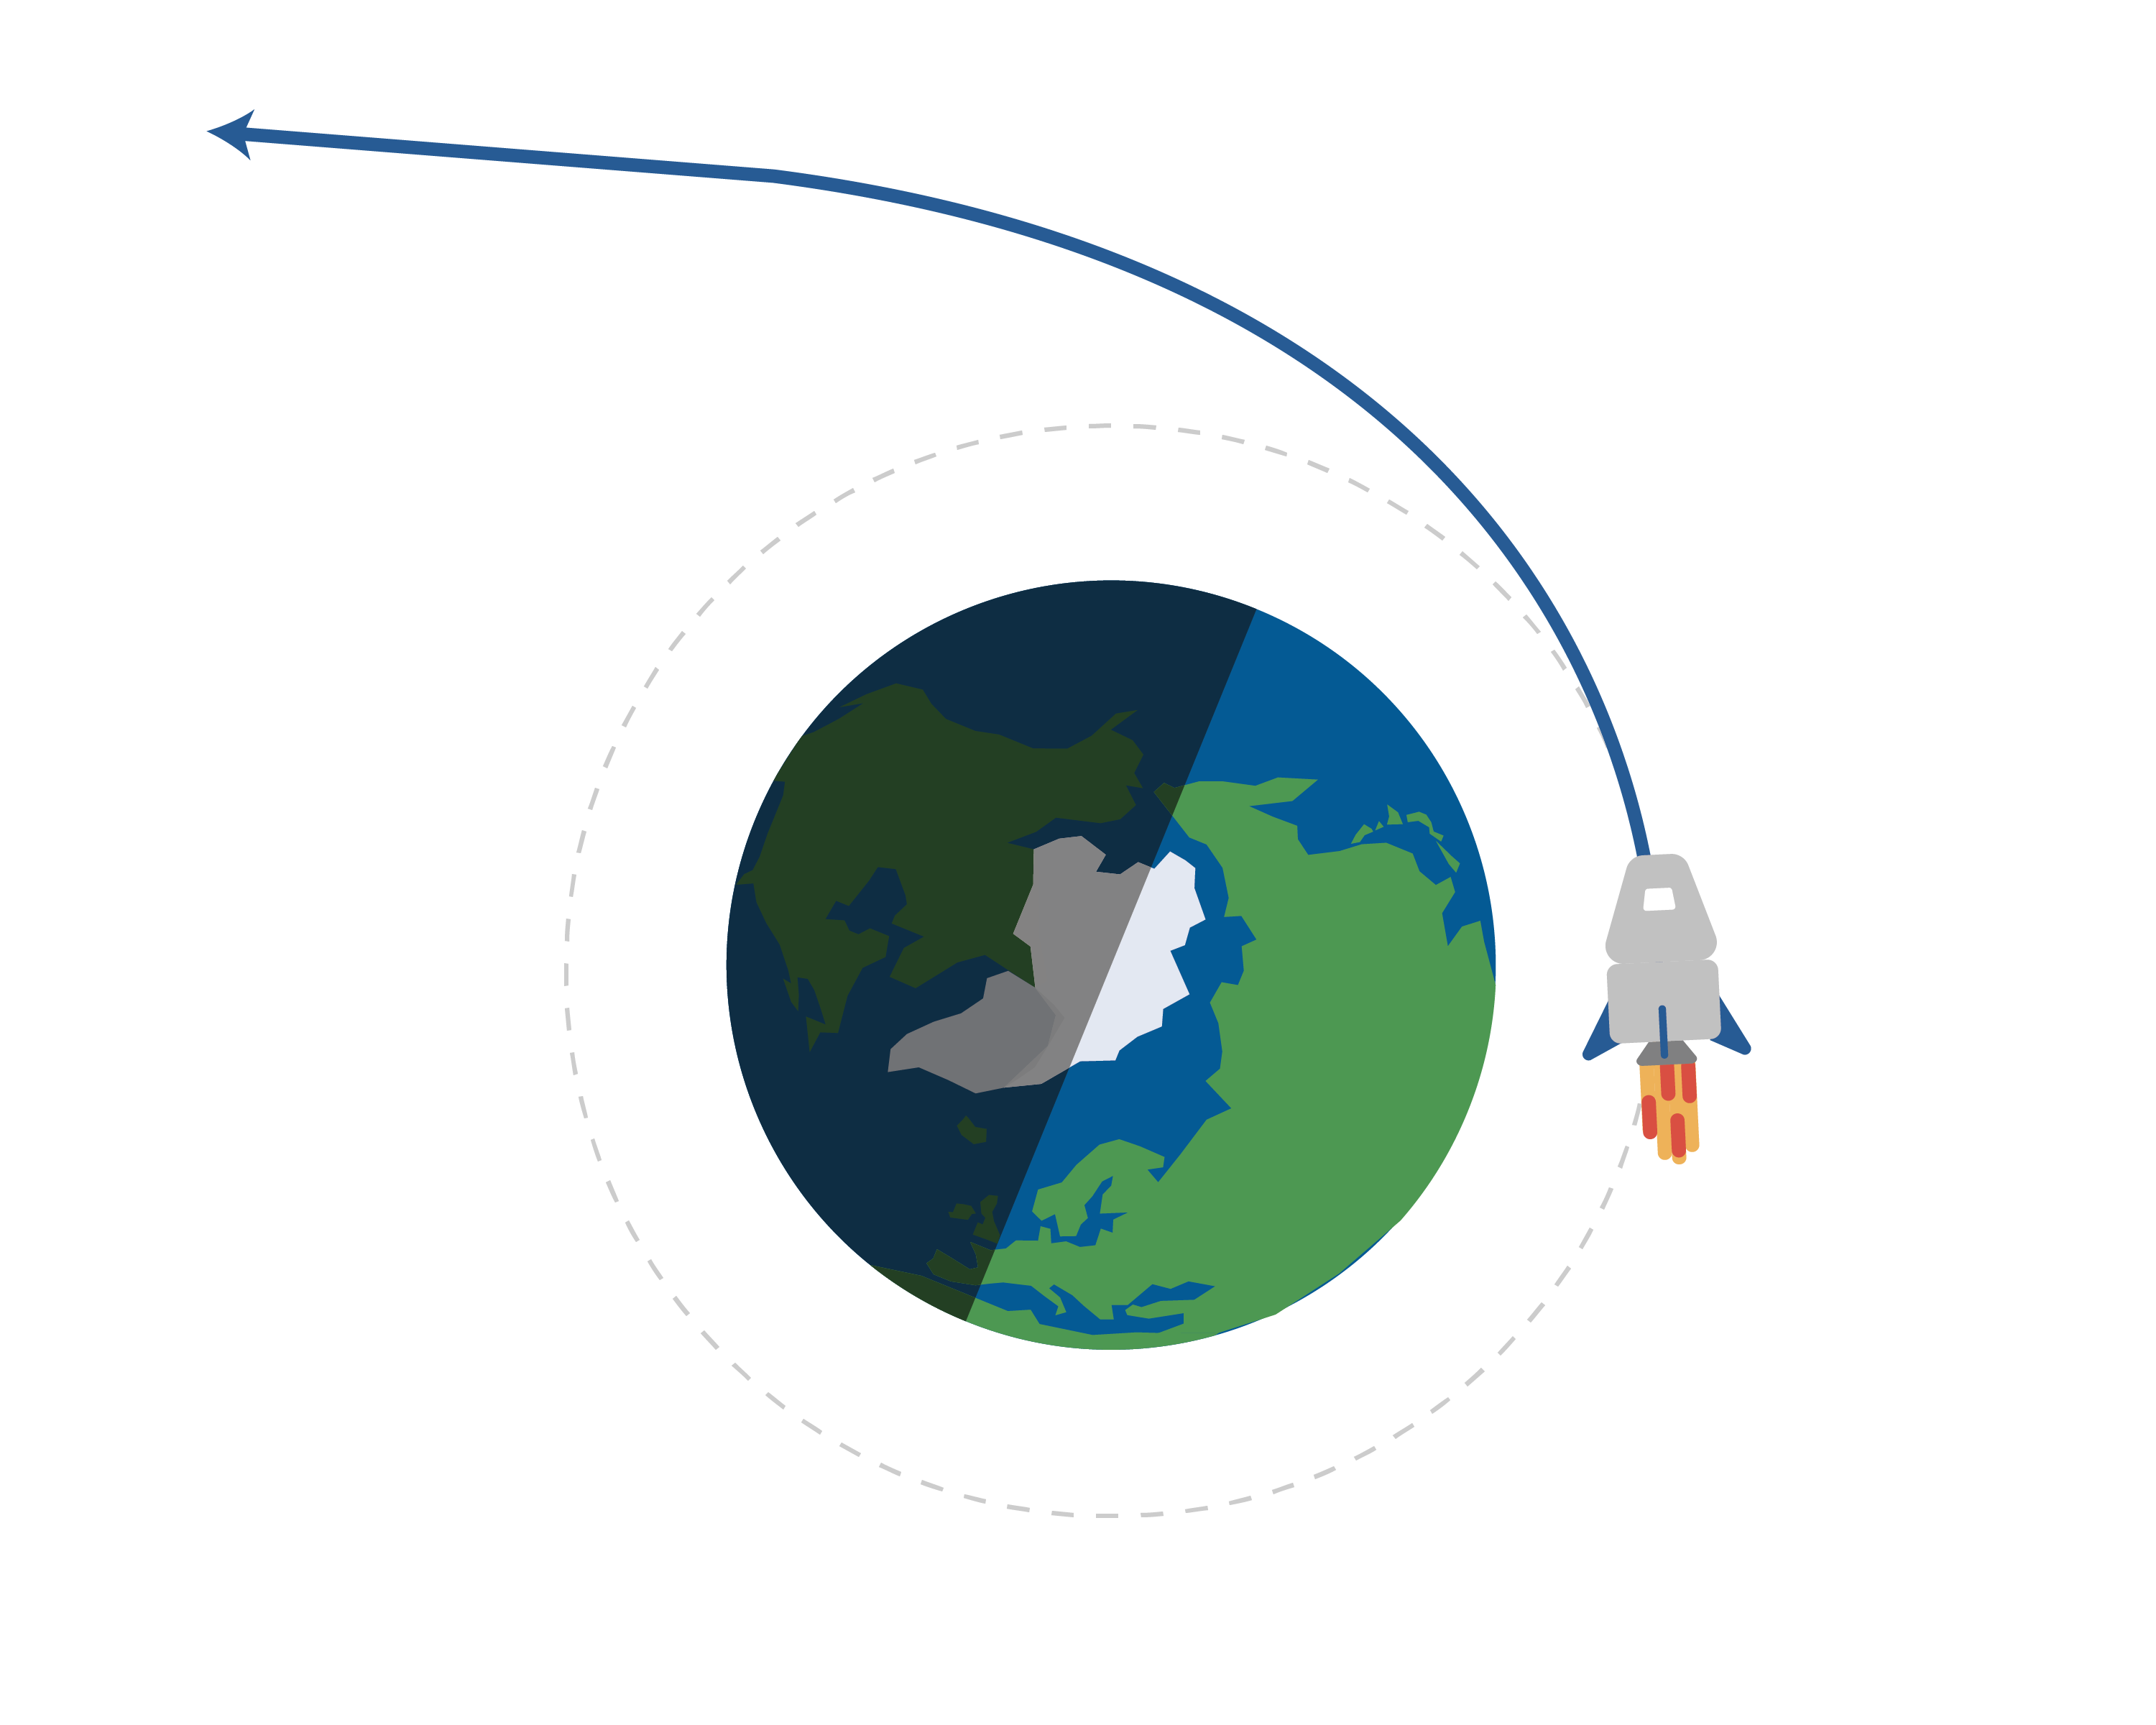
\includegraphics[width=.75\textwidth]{escape.png}
    \caption{A satellite can reach a speed at which it "escapes" earth's orbit (centripetal force).}
    \label{fig:escape}
\end{figure}


%FIXME reintroduce/mention gravitation (outside of earth gravity) here? Would be good